% !TeX root = ../thuthesis-example.tex


%\chapter{论文主要部分的写法}
\chapter{Introduction}

\section{Background}
Representation learning \cite{bengio2013representation}, especially deep representation learning (or deep learning, DL), has become one of the most popular techniques since \citet{krizhevsky2012imagenet} developed a powerful deep neural network (DNN) that can significantly outperform shallow methods on ImageNet \cite{deng2009imagenet}. After that, DNN based methods have thrived in various machine learning domains, including computer vision \cite{simonyan2014very}, natural language processing \cite{kim-2014-convolutional}, recommendation \cite{cheng2016wide}, reinforcement learning \cite{silver2016mastering}, and so on. These works make a substantial progress in building better artifical intelligence (AI) applications by DNN. However, it remains elusive why DNN gains so much improvement with adding more layers of representations. This question encourages us to think of opening the black box of DNN.


\begin{figure}[t]
  \centering
  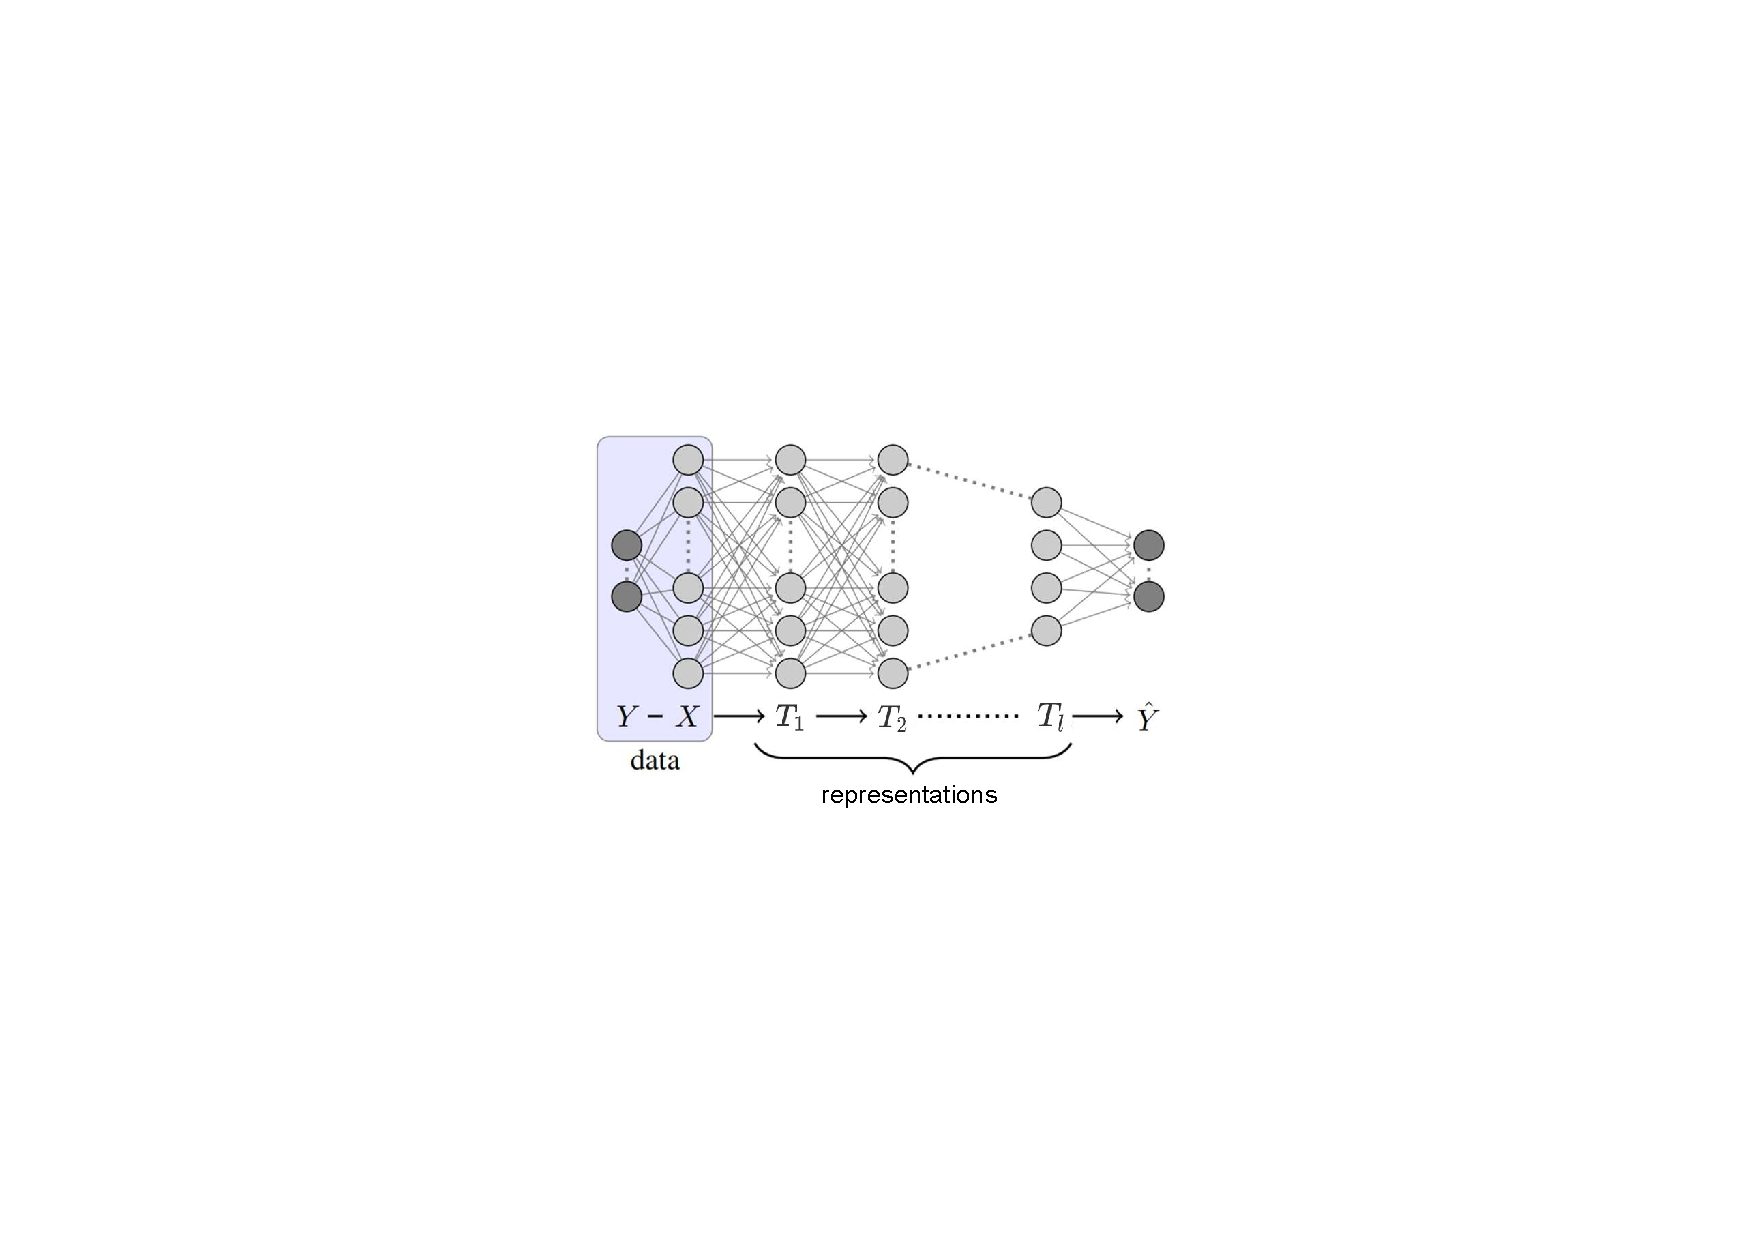
\includegraphics[width=0.6\linewidth]{fig1.pdf}
  \caption{A hierarchy of representations in DNN is formulated as a Markov chain, reproduced from \inlinecite{tishby2015deep}.}
  \label{fig:hierarchy_dnn}
\end{figure}






\section{Literature review}
\lipsum[1]

\section{Thesis structure}
\lipsum[1]

